% Part 1: Detecting DNA-bound RecB molecules
\section*{Results}

\subsection*{Imaging DNA-bound RecB molecules}

\begin{figure*}[htbp]
\begin{center}
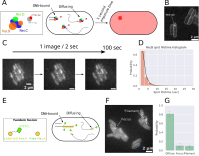
\includegraphics[width=\textwidth]{Figures/Fig1_endogenous.pdf}
\end{center}
\caption{Imaging DSB repair in live \textit{E. coli}. (A) Scheme of our experimental protocol. The RecB subunit of the RecBCD complex is fused to a Halo-tag, bound by the JF549 fluorescent dye. A long exposure time (1 sec) makes diffusing molecules appear as diffuse signal in the cell, while DNA-bound molecules are visible as bright, diffraction-limited spots. (B) Example image of a RecB spot (white arrow). (C) Example images of a timelapse acquisition (1 image every 2 sec for 100 sec). (D) Histogram of the lifetime of RecB spots (bars) fitted with a mono-exponential decay function ($y=a.e^{-k.t}$) (E) Scheme of our RecA imaging system (from \cite{Wiktor2021}). Free and fluorescently labelled RecA are present in equal amounts in the cell. (F) Example image of RecA imaging under endogenous DNA damage. RecA is diffuse in most cells, a RecA focus and a RecA filament are visible in two of the cells (white arrows). (G) Proportions of cells containing the different RecA structures (dots: individual datasets, bars: average between datasets).}
\label{Fig:endogenous}
\end{figure*}

%% Explain what we are trying to do (detect RecB binding to DNA)
%% Mention that bacteria experience endogenous damage
%% Explain the experiment principle, conclude with the fact that we are detecting RecB spots (SI control: no spots on the free Halo images)
To image Rec\-BCD in live \textit{E. coli}, we used a Halo-tag fusion to the RecB subunit, conjugated to the JF549 fluorescent dye (Figure \ref{Fig:endogenous}A). The fusion was previously used and characterised in the lab, ensuring specific one-to-one labelling of RecB molecules without adverse effects on the DNA repair process.\cite{Lepore2019a} To detect the binding of RecB to DNA, we applied the previously developed technique of localisation enhancement.\cite{Yu2006, Elf2007}  Since RecB is present at low copy numbers in \textit{E. coli} ($\sim$5 molecules per cell on average\cite{Lepore2019a}), imaging live cells with a long exposure time (1 second) made diffusing molecules appear as weak homogeneous signal in the cell, while DNA-bound molecules formed intense diffraction-limited spots (referred to throughout this article as RecB spots). (Figures \ref{Fig:endogenous}A, B) The complete absence of similar spots in cells expressing the free Halo-tag from a plasmid confirmed that these structures were specific to RecB (Supp. Figure \ref{SIFig:freehalo_image}). Seeing RecB spots in cells that were not exposed to an exogenous source of DNA damage was unsurprising, as these cells are still subject to occasional endogenous DNA damage. This can be due for example to collisions between the replication fork and DNA-bound proteins, and was previously reported to affect $\sim$18\% of cells per cell cycle.\cite{Sinha2018}

Acquiring short timelapse videos (50 images over 100 seconds, Figure \ref{Fig:endogenous}C) allowed us to measure the binding time of RecB on DNA. The resulting spot lifetime histogram was well-fitted by a mono-exponential decay model ($y=a.e^{-k.t}$, with a the fit amplitude and k the dissociation rate from DNA), consistent with a homogenous populations of fluorescent spots (Figure \ref{Fig:endogenous}D). The fitted spot lifetime was 1.5 sec $\pm$ 0.1. This prolonged imaging of the RecB-Halo fusion and quantification of DNA binding times was only possible thanks to the exceptional photostability of the JF549 dye, which displayed slow photobleaching and no blinking (Supp. Note \ref{note:dye_bleaching} and Supp. Fig. \ref{SIFig:dye_bleaching}). 

%% RecA makes foci and filaments
\subsubsection*{RecA forms foci and filaments}
One of RecBCD's purposes when processing a DSB is to facilitate the loading of the RecA protein on single-stranded DNA. To broaden our view of the repair process downstream of RecBCD, we imaged a tandem fusion of RecA with the fluorescent protein SYFP2 (Figure \ref{Fig:endogenous}E).\cite{Wiktor2021} Based on the fluorescence distribution in the cells, we identified three states of RecA: diffuse, forming a bright focus, or forming an elongated filament (Figure \ref{Fig:endogenous}F). Because of the large diversity of shapes observed, especially for RecA filaments, the detection of RecA structures by rule-based algorithms was challenging. Therefore, we designed and trained a deep-learning algorithm capable of classifying individual cells based on the three types of structures cited above (see Methods and Supp. Figure \ref{SIFig:object_class}). This allowed us to quantify the fraction of cells where RecA is freely diffusing to 81\% $\pm$ 6, RecA foci to 10\% $\pm$ 4, and RecA filaments to 9\% $\pm$ 2 (Figure \ref{Fig:endogenous}G). This is consistent with a minority of cells experiencing DNA damage, and being engaged in the repair process.

% Part 2: Separating genuine RecB binding events
\subsection*{Finding DNA binding events}

\begin{figure*}[htbp]
\begin{center}
\includegraphics[width=\textwidth]{Figures/Fig2_cipro_nSpots.pdf}
\end{center}
\caption{RecB DNA binding under ciprofloxacin exposure. (A) Example images of RecB throughout an acquisition. A short timelapse (100 sec) is acquired at a different position every 2 min for 75 min. (C) Number of RecB spots per cell area, at 0 and 30 ng/mL ciprofloxacin (panels) in cells expressing the Gam protein, or not (WT) (D) RecB spot lifetime histograms at 30 ng/mL ciprofloxacin, fitted with a bi-exponential decay model (black line, fit components showed as dashed lines). (E) Number of RecB spots per cell area, as a function of ciprofloxacin concentration (panels) and exposure time to the antibiotic (X-axis). Black dots represent measurements from individual datasets, and solid bars are the average between them.}
\label{Fig:nspots}
\end{figure*}

%% We add ciprofloxacin to increase the level of DNA damage
To gain more insight into DNA binding by RecB, we induced additional DSBs by adding ciprofloxacin to agar pads before imaging. Cells were left to settle down on the pad for 15 min, and then 50-frame timelapse videos were acquired at a rate of one position every 2 min (Figure \ref{Fig:nspots}A) for 60 min. This allowed us to quantify RecB binding at different time points ranging from 15 to 75 min after ciprofloxacin exposure.

%% RecB spot lifetime histograms change upon exposure to ciprofloxacin
%%% They are not well-fitted by a monoexponential decay (SI fig)
%%% We fit with a bi-exponential decay model
%%% Mention lifetimes/proportions, in table
Upon exposure to ciprofloxacin, the RecB spot lifetime histograms contained relatively more long-lived spots. Fitting with a mono-exponential decay model as in Figure \ref{Fig:endogenous}D did not account well for these long-lived spots (Supp. Figure \ref{SIFig:monoexp_fits}), especially at the higher ciprofloxacin concentrations. This suggested that the new long-lived spots that appeared under exposure to ciprofloxacin corresponded to a new population of RecB spots, that had a slower dissociation rate from DNA than the ones observed under endogenous damage. Indeed, fitting with a bi-exponential decay model ($y = a_1.e^{-k_1.t} + a_2.e^{-k_2.t}$) accounted much better for the longer-lived RecB spots (Figure \ref{Fig:nspots}). The bi-exponential fit outlined two populations of spots, with different lifetimes: a short-lived one, with lifetimes ranging from 1.2 to 1.5 sec, and a longer-lived one, with lifetime between 5 and 10 sec (Table \ref{tab:fit_results}). Even though the short-lived spots always represented a majority of events ($>$ 90\% of the spots), the proportion of long-lived spots tended to increase under higher ciprofloxacin exposure (from 3.4\% $\pm$ 0.9 under 3 ng/mL ciprofloxacin to 7.5\% $\pm$ 2 under 30 ng/mL ciprofloxacin).

\begin{table}[htbp]
    \centering
    \begin{tabular}{llll}
        \toprule
         &  & Lifetime (sec) & Proportion (\%) \\
        Ciprofloxacin & Type &  &  \\
        \midrule
        \multirow[t]{2}{*}{0} & Short & 1.24 $\pm$ 0.2 & 97.38 $\pm$ 0.72 \\
         & Long & 7.15 $\pm$ 1.2 & 2.62 $\pm$ 0.72 \\
        \cline{1-4}
        \multirow[t]{2}{*}{3 ng/mL} & Short & 1.17 $\pm$ 0.16 & 96.6 $\pm$ 0.89 \\
         & Long & 5.54 $\pm$ 1.06 & 3.4 $\pm$ 0.89 \\
        \cline{1-4}
        \multirow[t]{2}{*}{10 ng/mL} & Short & 1.18 $\pm$ 0.14 & 94.91 $\pm$ 0.8 \\
         & Long & 6.53 $\pm$ 1.36 & 5.09 $\pm$ 0.8 \\
        \cline{1-4}
        \multirow[t]{2}{*}{20 ng/mL} & Short & 1.39 $\pm$ 0.18 & 95.78 $\pm$ 0.83 \\
         & Long & 9.21 $\pm$ 1.14 & 4.22 $\pm$ 0.83 \\
        \cline{1-4}
        \multirow[t]{2}{*}{30 ng/mL} & Short & 1.49 $\pm$ 0.23 & 92.48 $\pm$ 1.95 \\
         & Long & 9.83 $\pm$ 1.74 & 7.52 $\pm$ 1.95 \\
        \bottomrule
        \end{tabular}
    \caption{Parameters derived from the spot lifetime histogram fits (Figures \ref{Fig:endogenous}D and \ref{Fig:nspots}B). The lifetime was calculated as the inverse of the fitted dissociation rate. Values are given as the mean $\pm$ standard deviation over 3 independent datasets.}
    \label{tab:fit_results}
\end{table}

%% To check what these two populations are, we use the Gam protein to prevent DNA binding and fit with the same model
%%% Short-lived population stays, long-lived one is removed
%%% Interpretation: because of its size, the RecBCD-Halo-Gam complex can sometimes form spots (SI Note + SI Fig if any), which creates short spots
%%% Therefore, we are unable to detect short DNA binding events, but we can confidently detect longer DNA binding events
To determine whether both short- and long-lived spots resulted from RecB binding to DNA, we measured RecB spots lifetime in the presence and absence of ciprofloxacin while over-expressing the Gam protein of phage $\lambda$ from a plasmid. The Gam protein was previously shown to bind in place of DNA on the RecBCD complex\cite{Wilkinson2016}, and its overexpression is expected to abolish RecBCD binding to DNA. Accordingly, cells that over-expressed Gam and were exposed to high ciprofloxacin (30 ng/mL) showed little elongation compared to cells that did not overexpress Gam (Supp. Figure \ref{SIFig:Gam_cell_length}). The resulting RecB spot lifetime histograms showed a near-complete disappearance of the long-lived spots, while short-lived ones were still present (Figure \ref{Fig:nspots}C). This was confirmed by fitting the histogram with our bi-exponential decay model, which found proportions of long-lived spots ($\sim$3\%) similar to those in wild-type cells that were not exposed to ciprofloxacin (2.6\%, Table \ref{tab:fit_results}). This confirmed that (i) long-lived RecB spots correspond to RecB molecules that have bound to DNA, and (ii) short-lived RecB spots can result from other causes than short-lived DNA binding (Supp. Note \ref{note:spurious_spots}).

%% We define a threshold (10 sec) above which no spots are observed in the Gam control (95% confidence). Any spots longer than 10 sec are expected to correspond to a DNA binding event.


% Part 3: There are two regimes of DNA repair for ciprofloxacin-induced damage
\subsection*{There are two regimes of DNA repair for ciprofloxacin-induced damage}

\begin{figure*}[htbp]
\begin{center}
\includegraphics[width=\textwidth]{Figures/Fig4_cipro_30ngmL.pdf}
\end{center}
\caption{}
\label{Fig:high_cipro}
\end{figure*}


%% At high cipro (above MIC, 20-30 ng/mL) we see a strong accumulation of RecB spots in the cell
%% Moreover these spots are centred in the cell (consistent with SOS/RecN-induced chromosome compaction)
Upon exposure to the higher cipro\-floxacin concentrations (20 and 30 ng/mL), the proportion of cells that contain at least one RecB spot increased (Supp. Figure \ref{Fig:high_cipro}A). This hints at an accumulation of repair intermediates in cells that are exposed to large amounts of DNA damage. Furthermore, whereas at low ciprofloxacin concentrations (0, 3, 10 ng/mL) RecB spots were found throughout the cell, at higher concentrations they appeared more centred in the cell (Figure \ref{Fig:high_cipro}B). This is consistent with RecN-dependent, SOS-induced compaction of the bacterial chromosome upon DNA damage, as has been previously reported (cite RecN paper).

%% We also see a strong accumulation of RecA filaments (RecA foci seem to be transient and their number decreases over time)
Simultaneously with the increase in the number of RecB spots, RecA filaments became visible in a large number of cells (Figure \ref{Fig:high_cipro}C). After one hour of exposure to ciprofloxacin, the proportion of cells that contained a RecA filament was $\sim$40\% at 20 ng/mL ciprofloxacin, and $\sim$60\% at 30 ng/mL (Figure \ref{Fig:high_cipro}D). RecA foci on the other hand seemed to form quickly following ciprofloxacin exposure (present in $\sim$40\% of the cells after 15 min of exposure to 30 ng/mL ciprofloxacin) and come back to endogenous damage level after $\sim$1 hour. Taken together, these results show that RecA foci are transient structures in the repair process that do not accumulate under high DNA damage, whereas RecA filaments do accumulate, presumably when the homologous sequence cannot be found.

%% Conclude: there are two regimes of DNA repair for ciprofloxacin-induced damage:
%% 1. Sub-lethal cipro concentrations, where repair structures are formed then disappear as damage gets repaired
%% 2. Lethal concentrations of cipro, where repair structures are formed and accumulate over time while the cell fails to repair its DNA
In these experiments, we can observe two regimes of DNA repair after ciprofloxacin exposure. At sub-MIC ciprofloxacin concentrations (0, 3, 10 ng/mL), repair structures such as RecB spots and RecA filaments form transiently and disappear as the damage gets repaired. At higher ciprofloxacin concentrations (20, 30 ng/mL), the DNA damage caused is more extensive, and repair structures are formed and accumulate over time while the cell fails to repair its DNA, ultimately leading to cell death.


% Part 5: Mutants in the repair pathway
\subsection*{RecB dissociation depends on RecA loading}

\begin{figure*}[htbp]
\begin{center}
\includegraphics[width=\textwidth]{Figures/Fig5_mutants.pdf}
\end{center}
\caption{}
\label{Fig:mutants}
\end{figure*}

%% There are more RecB spot per cell area in the mutants (Fig 5A). Because the level of DNA damage (endogenous or ciprofloxacin) is the same, we have to conclude that this represents slower dissociation of RecB from DNA.
%%% drecA has more RecB spots, both with and without cipro. This means that RecA plays a role in RecB dissociation from DNA, presumably associated with RecA loading
Compared to wild-type cells, all tested mutants showed a higher number of RecB spots per cell area (Figure \ref{Fig:mutants}A). Since the level of DNA damage (endogenous or 30 ng/mL ciprofloxacin) was the same for wild-type and mutant cells, this higher number of RecB spots must represent a slower dissociation of RecB from DNA. In light of this, the increased number of RecB spots in the \dreca\ mutant suggests that RecA plays a role in RecB dissociation from DNA, presumably associated with RecB's role in RecA loading.

%%% RecB1080 has even more spots than drecA. This means something else than RecA loading deficiency must make RecB dissociation difficult. We can hypothesise that it's RecB nuclease deficiency, which might make it hard for RecBCD to come off the DNA once it's threaded in
The \teneighty\ mutant is deficient in RecA loading, and nuclease activity.\cite{} It can bind DSBs and unwind the DNA duplex, but does not degrade the unwound strands. Even though it is unable to directly promote RecA loading, this still happens through an alternative pathway implicating RecJ and RecFOR.\cite{} Both in the presence and absence of ciprofloxacin, the \teneighty\ mutant shows more RecB spots than the WT or the \dreca\ mutant (\ref{Fig:mutants}A). This suggests that the increased lifetime of \teneighty\ on the DNA is not only due to its deficiency in RecA loading but also to the absence of its nuclease activity. Unwinding DNA without digesting it might make dissociation more challenging due to the DNA strands threading through the RecBCD complex.

%%% Entirely removing RecA in a 1080 background increases again the number of RecB spots per cell area, i.e. reduces the dissociation rate. This means in 1080 single-mutant, RecA still helps to dissociate RecB, presumably thanks to its loading by RecFOR.
Finally, the \dreca-\teneighty\ double-mutant displays a slight increase in the number of DNA-bound RecB per cell area compared to the \teneighty\ single-mutant (\ref{Fig:mutants}A). This means that in the \teneighty\ single-mutant, RecA still helps RecB to dissociate, presumably thanks to its loading by RecFOR.

%% RecB spots in ΔrecA and/or 1080 background in the presence of ciprofloxacin are not centred as in WT.
%%% In ΔrecA there is no centring and even a slight "exclusion" of spots from the centre of the cell. This confirms the involvement of the SOS response in RecB spot centring.
Upon addition of high concentrations of ciprofloxacin (20-30 ng/mL), DNA-bound RecB molecules were mainly found in the centre of the cell (Figure \ref{Fig:high_cipro}A), which we attributed to SOS-dependent compaction of the bacterial chromosome. In the \dreca\ mutant at 30 ng/mL ciprofloxacin, DNA-bound RecB were found throughout the cell, with a slightly lower density towards the centre (Figure \ref{Fig:mutants}C). This pattern is similar to what would be expected of a DNA-bound protein in the absence of chromosome compaction (cite an Achilles article here?). This observation reinforces the idea that the centring of DNA-bound RecB observed in the wild-type under high ciprofloxacin depends on the SOS response.

%%% In 1080 there is no centring, but also no exclusion from the centre of the cell. This might correspond to a "mixed" population, where only a few spots get centred due to the delay in the SOS response
Interestingly, in the \teneighty\ mutant a more even distribution of DNA-bound RecB is observed. The density of bound molecules is not reduced at the centre of the cell, as was observed in the \dreca\ mutant (Figure \ref{Fig:mutants}C). This could be attributed to partial or delayed chromosome compaction, due to the largely reduced efficiency of RecA loading in the \teneighty\ mutant.

%%% In the double-mutant spots are again excluded from the cell centre, similarly to ΔrecA single mutant. This makes sense, as there will also be no SOS response in the double-mutant.
Finally, in the \dreca-\teneighty\ double-mutant, DNA-bound RecB molecules seem to adopt a similar phenotype to the \dreca\ single-mutant, where the density of molecules is reduced at the centre of the cell, consistent with a complete absence of SOS induction, and therefore no chromosome compaction.

